\subsection{Source-Disjoint Pilot and Parameter Sensitivity}
\label{sec:independent}
\subsubsection{A source-disjoint pilot and a separate development sweep}
Tables report source-referenced pixel measurements; evaluation provenance is documented in Appendix~\ref{app:evaluation-provenance}.

We evaluate five methods on 24 PIE-Bench sources with two seed slots per source. Selection used a fixed SHA256 ranking and category round-robin rule, excluding the six historical development sources; the first four categories contribute three sources each and the other six two each. The pilot sources subsequently inform development, including the ten-source support and memory ablations below. A separate parameter sweep uses the historical six-source, seven-task development set.

The automatic configuration, AUTO\_DETAIL, uses the same unfiltered regional update and online budget coefficient $a=0.25$ as Eq.~\eqref{eq:soft-support}. Its mask is computed solely from source-image contrast. After grayscale area resizing to the latent grid, absolute horizontal and vertical differences are summed, smoothed with a $5\times5$ average, thresholded at the image's 75th percentile, and smoothed again. This procedure selects detailed image regions. It uses neither an object segmenter nor a target instruction. Official PIE edit masks are reserved for evaluation. Memory remains active in steps 0--6 with gate one and all-image query coverage.

The four comparators are global quarter-strength correction with memory (U25\_KV), RF-Inversion with maximum $\eta=0.3$ (ETA03), FlowEdit N26, and the released RF-Edit adapter. FlowEdit uses 28 scheduler nodes, $n_{\max}=26$, $n_{\min}=0$, one noise sample, and source/target guidance 1.5/5.5. The RF-Edit adapter uses 25 second-order steps per direction, 20 injection steps, and guidance 1/5; its configuration is kept fixed across sources. It uses 100 transformer evaluations and is deterministic for these inputs. Deterministic repeats are aggregated within source; record-level details appear in the provenance appendix.

\subsubsection{Metric support and source-level inference}
The independent cohort evaluates edit-region and preservation-region MAE using the official PIE mask and its complement. Five sources have an empty preservation complement, yielding 19 sources and 38 outputs per method for preservation MAE. Edit-region MAE uses all 24 sources. Larger edit-region departure measures a larger pixel change; achievement of the requested transformation is a separate outcome.

The archived independent-cohort NCC uses the whole image. The crop spans the image boundary, so only zero displacement is valid in the shift search. Fixed and shifted NCC are consequently identical. This metric has a different support from the local pattern NCC in the development tables. Tables report those two scopes separately.

Paired differences match source, task, and seed, averaging repeated observations within source before 20,000 source-bootstrap resamples. Two-sided sign-flip tests use 20,000 draws with plus-one correction and Holm adjustment across four comparators within each metric. The intervals and tests are exploratory. The accompanying qualitative record covers all 48 pilot sheets.

\begin{table*}[t]
\centering\small
\caption{Independent-source pilot: 24 new sources and 48 output records per method. NCC is whole-image source correlation. Preservation MAE covers 19 sources with nonempty preservation masks; edit-region MAE covers all 24. Arrows apply to source retention within the named support. Edit-region departure has no quality arrow. Runtime is recorded synchronized execution time. RF-Edit values describe the released adapter and operating point.}
\label{tab:independent}
\begin{tabular}{lrrrrrr}
\toprule
Method & Whole-image NCC $\uparrow$ & Preservation MAE $\downarrow$ & Edit-region MAE & NFE & Time (s) & Outputs\\
\midrule
ETA03 & 0.6905 & 0.1135 & 0.1471 & 56 & 40.12 & 48\\
U25\_KV & 0.7464 & 0.1093 & 0.1400 & 91 & 43.67 & 48\\
AUTO\_DETAIL & 0.5995 & 0.1627 & 0.1790 & 91 & 44.29 & 48\\
FlowEdit N26 & 0.6879 & 0.1099 & 0.1615 & 52 & 31.20 & 48\\
RF-Edit adapter & 0.9814 & 0.0216 & 0.0302 & 100 & 46.69 & 48\\
\bottomrule
\end{tabular}
\end{table*}

\subsubsection{Automatic contrast routing increases unintended change}
Table~\ref{tab:independent} shows a transfer gap. AUTO\_DETAIL minus U25\_KV gives a whole-image NCC difference of $-0.14685$ and preservation-MAE difference of $+0.05338$, with source-bootstrap intervals $[-0.21115,-0.09307]$ and $[0.03767,0.06833]$. Relative to FlowEdit N26, the differences are $-0.08842$ in NCC, with interval $[-0.16775,-0.01004]$, and $+0.05278$ in preservation MAE, with interval $[0.03113,0.07455]$. Figure~\ref{fig:independent-effects} includes all four comparisons.

These results locate the problem more precisely than whole-image similarity alone: the additional departure includes pixels that the benchmark marks for preservation. The source-only contrast support also contains edges of content explicitly requested to change and leaves smooth retained content weakly constrained. This mask-selection explanation motivates the next controlled intervention; it is distinct from the measured preservation error itself.

\begin{figure*}[t]
\centering
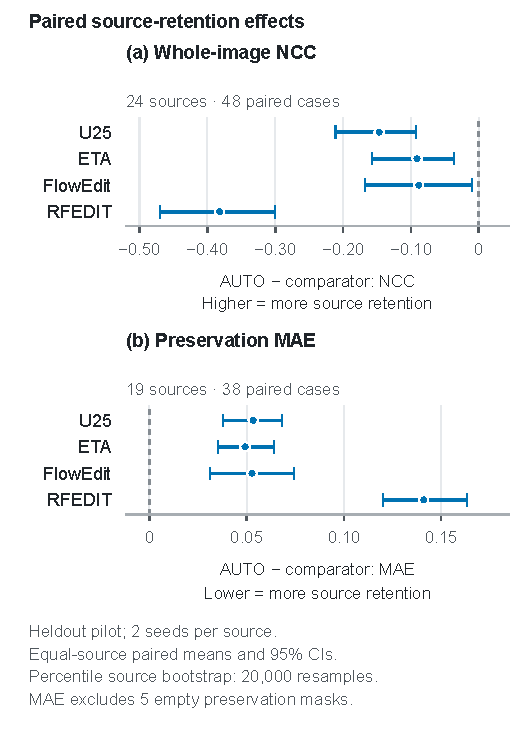
\includegraphics[width=.96\textwidth]{figures/r81_paired_effects.pdf}
\caption{AUTO\_DETAIL minus each comparator on new sources. Points are equally weighted source-level paired means; bars are percentile 95\% source-bootstrap intervals. NCC uses 24 sources; preservation MAE uses the 19 sources with nonempty preservation complements. These measurements describe source retention.}
\label{fig:independent-effects}
\end{figure*}

RF-Edit has the strongest source correlation and edit-region departure of 0.030. Its illustrated color, deletion, replacement, and style outputs remain close to the source scene. These observations characterize the recorded operating point; the adapter follows the official default injection schedule, with implementation provenance in Appendix~\ref{app:evaluation-provenance}.

\subsubsection{Visible edits and remaining semantic failures}
Figure~\ref{fig:independent-examples} presents two visible edits and two failures selected for illustration. AUTO\_DETAIL changes the kitten toward pale yellow while retaining the patterned blanket. In the deletion example, the foreground olives disappear and the pouring action remains, alongside changes to the bowl and setting. In the highway example, vehicles remain despite the request for boats. In the style example, overlapping child faces appear and the requested crayon rendering remains weak. The full per-seed observations also record changes in subject count, geometry, and surroundings. These image-specific observations explain why edit achievement, identity, preservation, and artifacts are separate evaluation dimensions.

\begin{figure*}[t]
\centering
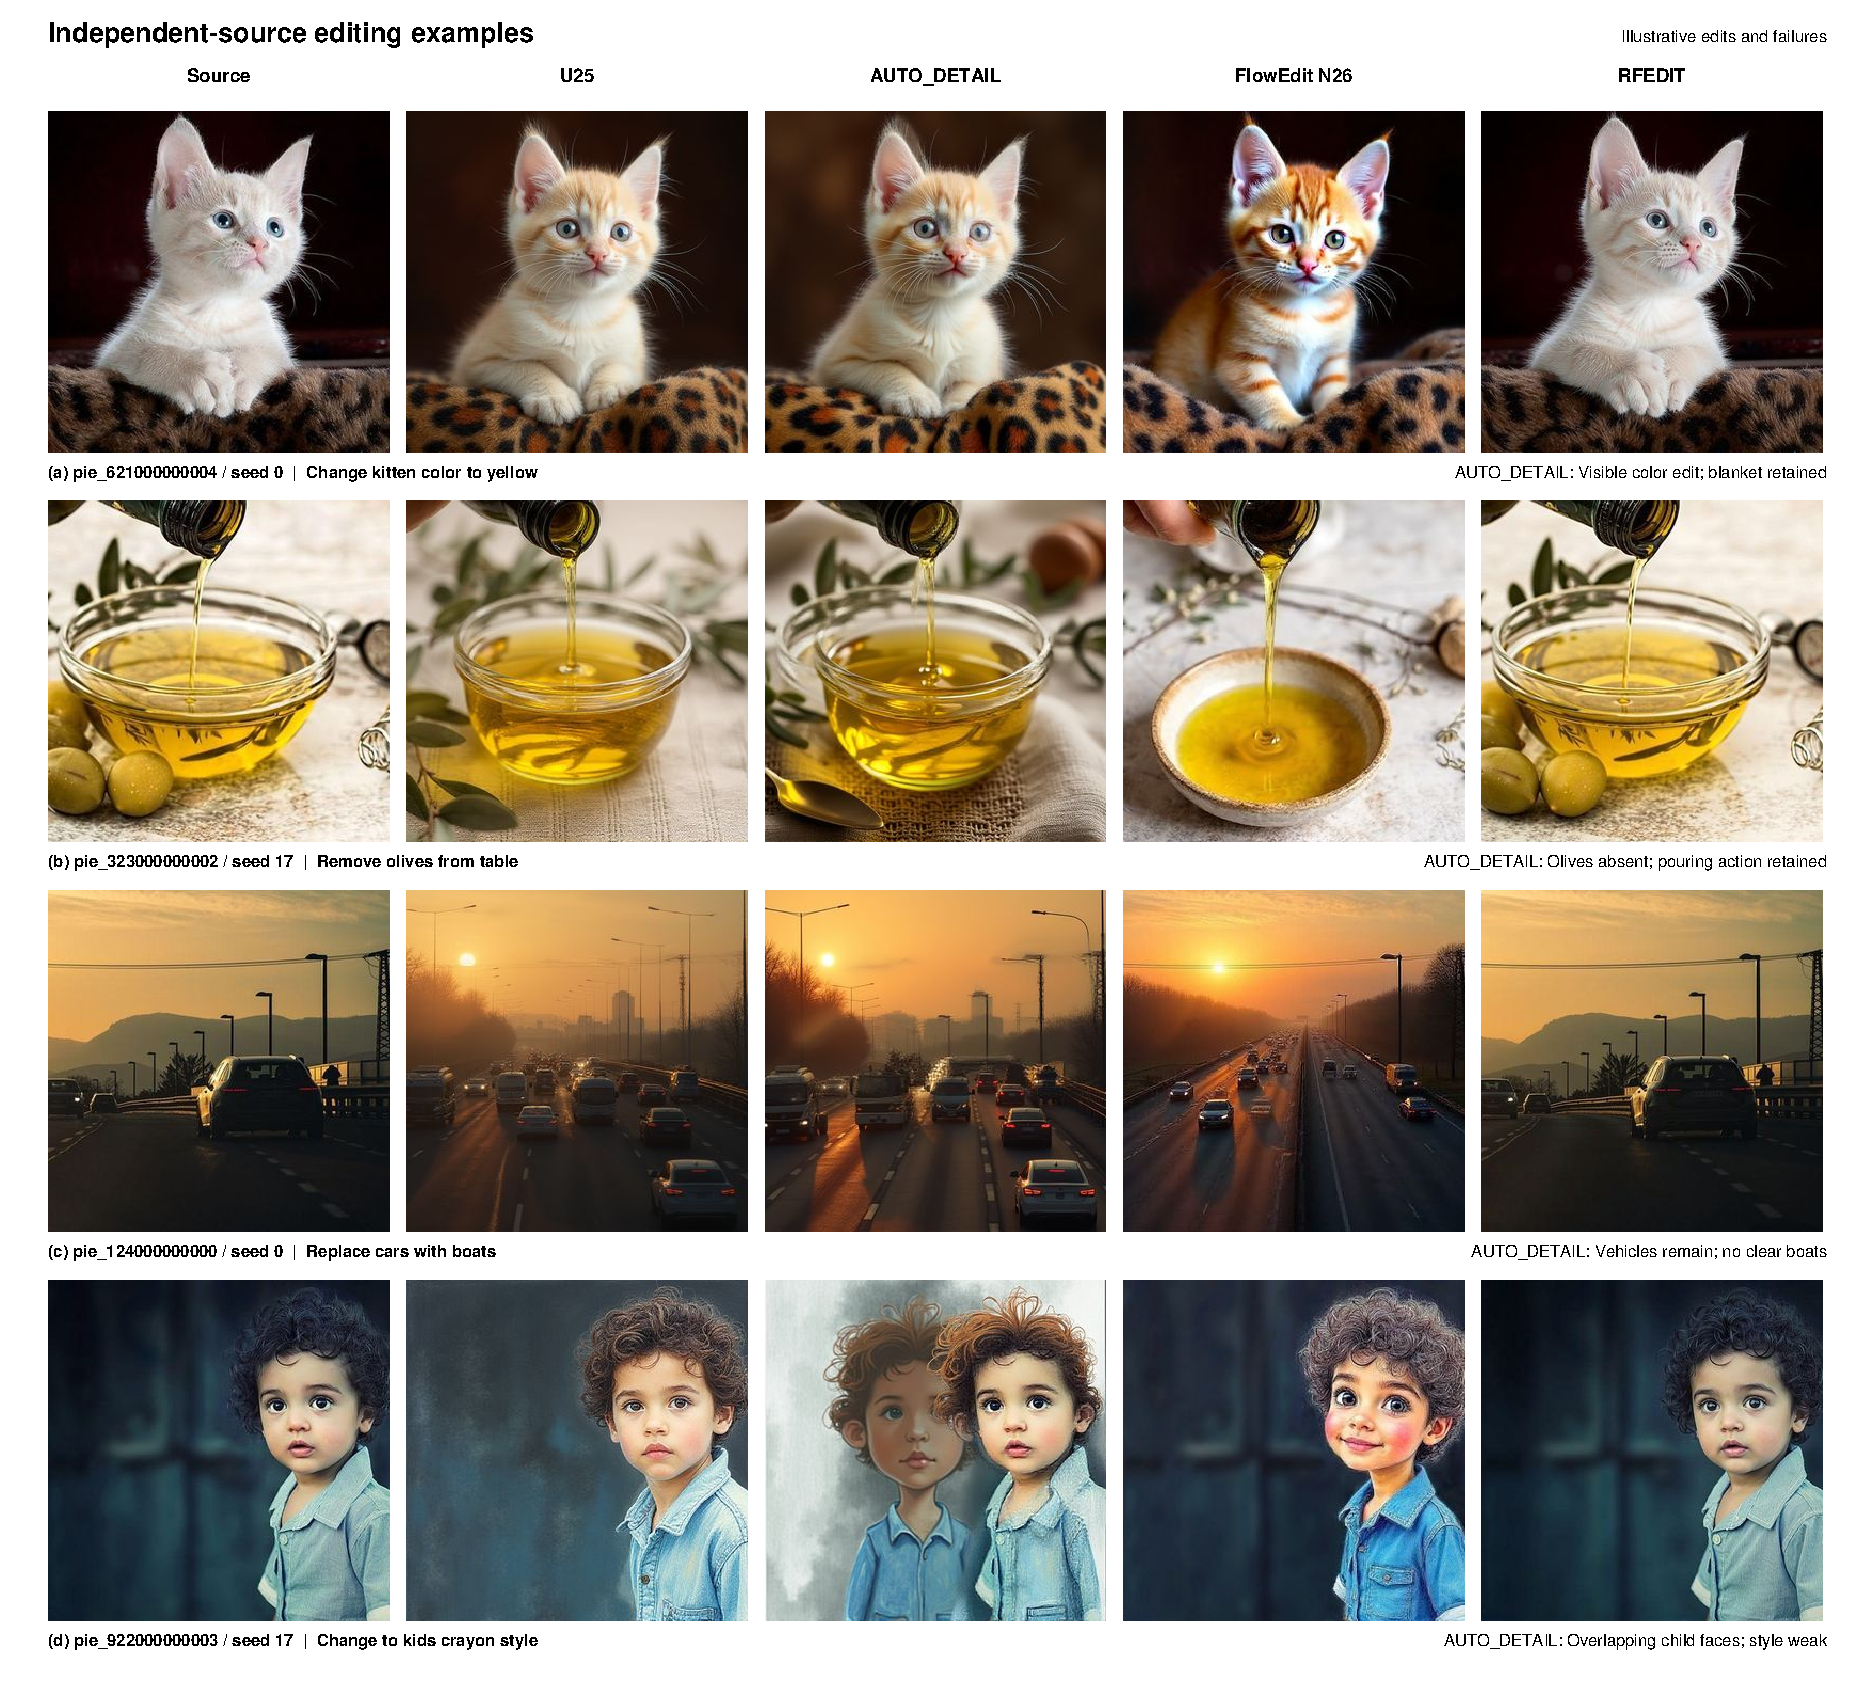
\includegraphics[width=.98\textwidth]{figures/r81_heldout_examples.pdf}
\caption{Independent-source examples with fixed prompts and seeds across methods. Rows show kitten recoloring, olive removal, car-to-boat replacement, and a crayon-style request. The first two illustrate visible requested changes with varying source retention; the last two illustrate missing replacement and duplicated geometry. Figure selection is qualitative, and no success rate is inferred from these four examples. All 48 sheet observations are retained in the accompanying CSV.}
\label{fig:independent-examples}
\end{figure*}

\subsubsection{Development parameters control different outcomes}
\begin{table}[t]
\centering\small
\caption{Additional development sweep: 14 outputs per row from six sources and seven tasks. NCC is local pattern NCC$_{\pm6}$; background MAE is source departure. The baseline ONLINE25 arm is a frozen earlier result and is not rerun in this cohort.}
\label{tab:parameter-sweep}
\begin{tabular}{lrrr}
\toprule
Configuration & NCC & Background MAE & NFE\\
\midrule
Budget 0.15 & 0.5942 & 0.1698 & 91\\
Budget 0.35 & 0.8470 & 0.1639 & 91\\
Memory gate 0.5 & 0.7563 & 0.2362 & 91\\
First 3 memory steps & 0.6973 & 0.1934 & 87\\
ROI erosion 16 px & 0.6418 & 0.1694 & 91\\
ROI dilation 16 px & 0.8230 & 0.1625 & 91\\
Memory only & 0.3447 & 0.1760 & 63\\
Source-only attention read & 0.7790 & 0.1571 & 91\\
RF-Edit adapter & 0.9652 & 0.0225 & 100\\
\bottomrule
\end{tabular}
\end{table}

Increasing the manual-region budget from 0.15 to 0.35 raises local NCC from 0.594 to 0.847 with similar mean background departure. Expanding the manual ROI gives 0.823 NCC, compared with 0.642 after erosion. Both comparisons show that local strength and support coverage matter. The memory-gate 0.5 arm has greater background departure (0.236) and local NCC 0.756. Three memory steps save four transformer calls and yield NCC 0.697. Memory alone yields 0.345. These operating points distinguish retention, source departure, and cost; selecting a global editing configuration also requires task achievement.

The preservation-error increase occurs in 18 of the 19 eligible sources. Removing any single source leaves the mean increase between 0.050 and 0.058. Every category with an eligible preservation region has a positive mean difference. These source-level results locate the transfer failure beyond any single image or category.

The support ablation retains $a=0.25$, seven memory steps, and gate one while changing spatial allocation. ONLINE normalizes against uniform correction at each arm's own current state. The pilot's mean impulses are 0.259 for AUTO and 0.232 for U25, an 11.4\% difference; a shared coefficient therefore requires reporting realized impulse alongside normalization error.
